
\section{Capacity Increases Performance}
\label{sec:store}

In addition to relaxing the need for intermittent techniques, we find that
an increase in sensor energy capacity
%for the harvesting
%conditions and workloads we consider
achieves a significant return on sensor
reliability and capability in the face of variable energy income.  Higher
energy capacity allows higher energy capture during periods of abundant
harvestable energy.

%The clearest path towards increasing reliability in
%a resource-constrained, energy harvesting system is to increase the
%amount of available ambient energy that can be captured for use by the sensing
%applications. We show that for the sensor workloads and indoor lighting conditions
%described in \cref{sec:overview}, the efficiency of this ambient energy
%utilization is highly dependent on the size of the secondary energy store and
%that increasing the size of this store can greatly increase reliability
%of the system, especially in periods of energy drought. While this observation
%is unsurprising, we show that a small investment in rechargeable capacity
%yields a disproportionate return in reliability.

\subsection{Ambient Energy Utilization}
\label{sec:store:utilization}

Ambient energy is underutilized when it is not used to support the specified
sensing application. This may happen for two reasons: 1) the secondary
energy store is full but energy is still available for harvesting, and 2) the
sensor performs work based on its energy state rather than its application
goals. The first scenario is common for energy harvesting systems
presented in prior work, which charge up a capacitor and wait for an event
before sensing and sending, failing to capture all energy that may
have been harvested while their capacitor was full~\cite{campbellEnergy14}.
For an example of the second scenario, consider
systems that transmit a packet every time their energy storage capacitor
is full rather than saving this energy for use during periods of lower harvesting
potential~\cite{hesterFlicker17, colinReconfigurable18}. Another example of this are sensors in which the harvesting
rate is proportional to the sensed phenomena~\cite{debruin2013monjolo}.
While compelling for their simplicity, these sensors use
energy that could be saved and used
later for more useful and relevant tasks.
%to indicate the absence of energy or perform other tasks.

To explore ambient energy utilization as a function of storage size, we
model the charge-discharge patterns of idealized energy stores under
the harvesting conditions and workloads described in \cref{sec:overview}.
This modeling is primarily accounting for our first classification of
wasted energy, since our workload definitions \textit{do not} perform
tasks in response to available energy; instead they attempt to maximize the success
rates for the specified sensing tasks.
The results of this modeling are shown in \cref{fig:usage}. No matter
the amount of available energy, utilization increases as
storage capacity increases. For scenarios with low harvesting potential and high
power workloads, a sensor with at least 1\,mWh of storage can accomplish 100\% utilization.
%if the energy store
%approaches capacities on the order of 1\,mWh of capacity.
In cases of
high harvesting potential and low power workloads, utilization often
stops increasing before reaching 100\%. This
can be attributed to a small fraction of the available energy being sufficient
to fully support the sensing task.
%We note that even
Small increases in utilization
%can
%translate to significantly more absolute usable energy and
have significant impact on reliability and system lifetime.
\placefigure[t]{fig:reliability}

\subsection{Application Reliability}
\label{sec:store:reliability}

%We analyze the impacts of increased energy utilization on an application's
%reliability
We also model the ability of varying energy stores to meet our defined
sensing tasks and intensities. Our results are
%as well as parameters for those tasks (such as sensing period
%and event frequency),
shown in \cref{fig:reliability}. %shows this analysis, and
Similar to the results of \cref{sec:store:utilization}, we see marked
increases in performance when energy stores reach 1-10\,mWh
of capacity.
Simulations experience 100\% reliability for all but
the most energy constrained scenarios with high power workloads and
$\geq$2\,mWh of energy storage.
We also see that even when low capacity sensors
have large energy harvesting potentials and infrequent workloads, they experience low
reliability.
%Similarly, even for high period (less intense) workloads, low capacity sensors perform poorly.
%We also examine which workload period is practical for a given energy storage
%size and harvesting environment in \cref{sec:store:reliability}.
This is because they
do not have enough storage to keep sensing throughout the night.
%Unsurprisingly, designs with larger secondary
%sizes are capable of workloads with higher intensities. Best results are
%achieved with storage sizes of 0.3-3\,mWh, and a workload period
%greater than 30\,s.
%Configurations with small
%energy stores only achieve about 60\%
%If we instead
%look at detecting events from an occupancy sensor as in
%\cref{fig:reliability:eventsec}, which should favor
%smaller capacity configurations due to the correlation of ambient
%energy solar energy with occupancy, we see slight improvements.

Finally, we analyze the ability of different storage configurations to perform a
random, contiguous, higher energy task. We use a 100\,mJ (30\,\textmu Wh) event that is representative of a
50\,KB over-the-air code update. While this is larger than a code update would be
for simple programs,
%especially if one performs techniques such as differential patching,
we see in \cref{fig:reliability:otattc} that nearly all of the configurations with
0.28\,mWh of energy storage complete the task in the minimum time (5\,s). In comparison,
even reducing the amount of energy storage to match the amount of energy
required for the code updates causes significant latency. It is clear that
many of the updates for smaller energy storage configurations
do not complete for 1000-10,000\,s.
This aligns with the amount of time a sensor may sit
idle overnight waiting for solar power.
%before completing the task when more energy is available in
%the morning.

% Mayfly/Flicker
% - Timekeeper: 1 10uF 0805YD106KAT2A 0.09 @ 100 (equiv 0.03 @ 100) (0.023)
% - MCU: 1 22uF Not specified, but an AVX 1210 costs 0.44 @ 100 (equiv 0.079 @ 100) (0.025)
% - Acel 1 2.2uF EMK107BJ225KA-T 0.039 @ 100 (equiv 0.036 @ 100) (0.015)
% - BLE  1 47uF GRM31CR60J476ME 0.21 @ 100 (equiv 0.16 @ 100) (0.028)
% - HUM  1 15uF C2012X7S1A156M125AC 0.37 @ 100 (equiv 0.19 @ 100) (0.052)
% - Press 1 33uF C3216X5R0J336M130AC 0.44 @ 100 (equiv 0.38 @ 100) (0.034)
%
% Capybara
% - test 1: 400uF ceramic (4x100 0.31 equive @100) (0.043), 330uF tant (0.69 equiv @100) (0.24), 67.5 mF super (?? $21?, $2.42)
% - test 2: 300uF ceramic (3x100), 1100uF tant ($2.43) (0.62), 7.5 mF super ($2.42) (
% - test 3: 300uF cerami (3x100)c, 100uF tant ($0.28) (0.17), 7.5 mF super ($2.42)
%
% Gecko Power Supply
% - 5 TLJG227M004R3000 1.39 @ 100 (0.37 equiv, 0.16 ali)
%
% Wisp
% - 1 10uF ?? $0.05 @ 100
\begin{definefigure*}{fig:primary}
  \centering
  \begin{subfigure}{0.39\textwidth}
    \centering
    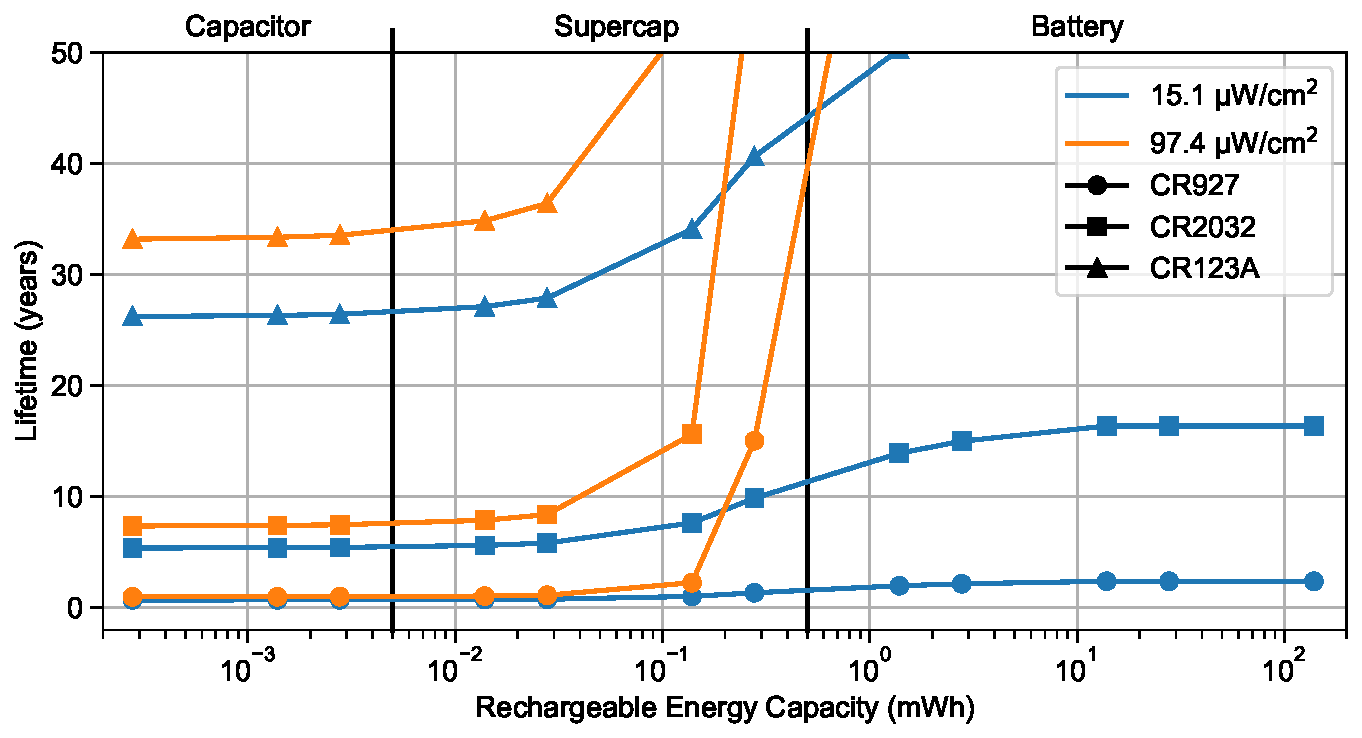
\includegraphics[width=0.85\linewidth]{figs/capacity/primary/sense_and_send_life_vs_sec_size}
    \caption{Periodic Application}
    \label{fig:primary:sensesec}
  \end{subfigure}
  \begin{subfigure}{0.6\textwidth}
    \centering
    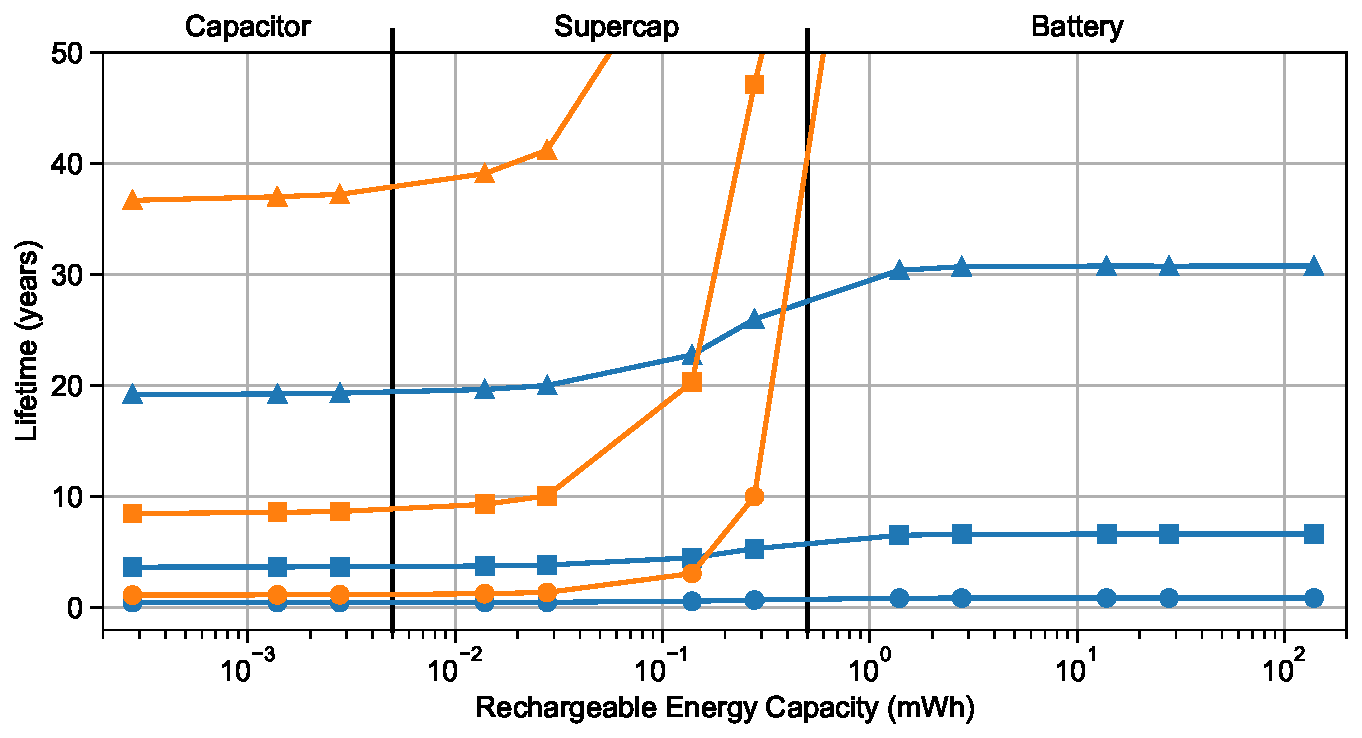
\includegraphics[width=0.85\linewidth]{figs/capacity/primary/door_occu_life_vs_sec_size}
      \caption{Reactive Application}
    \label{fig:primary:eventsec}
  \end{subfigure}
  \caption{
    \normalfont
    Estimated lifetime
    when varying secondary energy capacity for different harvesting scenarios
    and backup energy storage sizes. The periodic application's period
    is 30\,s and the reactive application events are scaled to
    represent a maximum of 2000 events per hour.
    %Harvesting scenarios and workloads
    %are described in \cref{sec:overview} and \cref{tab:rep}, and
    The backup
    sizes correspond to those found in common coin cell batteries:
    90\,mWh, 720\,mWh, 4500\,mWh for the CR927, CR2032, and CR123A respectively.
    As the ability to capture
    more harvested energy increases, the sensors lifetime increases.
    In some scenarios, expected
    lifetime becomes unbounded as the device is able to subsist entirely on harvested
    energy.
    %All scenarios experience substantial
    %increases in lifetime from increased secondary storage size.
    We see a 2-4x increase in lifetime estimates from the smallest to largest
    capacity simulated, if we only consider bounded results.
    We emphasize that
    these lifetime estimations are
    just estimations, and while we do model the 1\,\%/year leakage
    typical of coin cells, we do not consider the unknown
    physical degradation that would be experienced over decades of use.
    }
\end{definefigure*}

\section{Reliability Requires Backup}
\label{sec:primary}

Increasing secondary capacity greatly improves
reliability.
%for both periodic and reactive workloads.
However, some environmental
conditions and workloads do not reach 100\% reliability regardless of the size
of the secondary store.
%reactive workloads with large secondary
%capacities, some of the
Some results in \cref{fig:reliability}
appear to achieve perfect reliability, but still miss 0.1-2\% of events.
%with
%diminishing returns for increased secondary capacity.
%Additionally, some workloads
Others achieve well below 100\% reliability, %at the upper extents of storage capacity,
and simply require much more energy
than is harvestable. A backup energy store can increase reliability of a system
to 100\%, at the cost of a finite lifetime.
%In both of these case, further increasing secondary
%capacity does not improve reliability.
%and the desired application cannot rely soly on harvested power.
%and we expect that
%workloads which achieve slightly less than perfect reliability are experiencing
%a combination of brief harvesting droughts and high amounts of temporally local activity
%that push the local average power well above that of the average harvested power.
%While the second case may be solved with a sufficiently large secondary-cell, the
%diminishing returns of increasing secondary size and
%unpredictability of some reactive applications
%makes it difficult to rely solely on harvested power.

\subsection{Reliability Required}
\label{sec:primary:reliability}

We argue that 100\% reliability is a significant improvement over
even low failure rates with respect to reliability
%information
%for many applications
and simplicity due to the lack of intermittency.
%that is a consequence
%of reliability.
Many applications, especially human facing ones,
must be reliable to function, and research shows that unreliability
leads to frustration and %lack of
unwillingness to adopt automated solutions~\cite{brushHome11, edwardsHome01, shehanHome07}.
To use energy harvesting sensors for control or feedback of systems with potential
safety issues, inherent unreliability is intolerable.

Worse, intermittent system failures are difficult to detect %and mitigate
because there is no method for distinguishing between lack of energy
and an actual fault. While scheduled communication of current energy state
may help, this would be difficult for systems that only store enough
energy to perform a single operation such as Flicker~\cite{hesterFlicker17},
Gecko~\cite{yervaGrafting12}, and some configurations of
Capybara~\cite{colinReconfigurable18}.

Finally, it is more difficult
to program intermittent systems because programmers or the underlying
programming model must monitor and adapt to available energy with fine
granularity, both of which are non-trivial tasks.
These systems have little ability to correct for failures
even when they are detected.
%A reliable system has the ability to spend more short-term
%energy to correct for detected failures.

\subsection{Lifetime of a Backup Energy Store}
\label{sec:primary:lifetime}

To achieve 100\% reliability and avoid intermittency,
designs can utilize a backup energy store.
%that is pre-charged at the start of the
%node's life.
In instances where the rechargeable source is depleted, the system
can operate from the backup, masking the effects of variable energy income.
When the backup energy store is depleted, we consider the node's lifetime
to be complete, although it could continue
operating intermittently and with lower reliability. This energy store should
be a primary-cell, as they offer very low self-discharge, long shelf life, and
substantial energy density.
%This pre-charged energy store could be accomplished
%by either a large secondary-cell or a primary-cell, but to avoid increasing
%volume significantly this energy store will almost certainly manifest itself
%as a non-rechargeable battery.

An analysis of the reliable lifetime of a node with both energy
harvesting and a backup energy store is shown in \cref{fig:primary}.
%for
%both periodic and event based workloads.
We choose several backup energy
stores with energy equivalent to those found in several types of common
primary-cells. We see that with energy harvesting and a sufficiently
large secondary energy store, nodes can
achieve 100\% reliable lifetimes that exceed
what we can reasonably predict, especially for harvesting scenarios that
exceed the average power of the application. In these scenarios, %While this makes sense intuitively,
the inclusion of a backup energy store is critical %in these scenarios
to ensure reliability in uncharacteristically adverse conditions.
Even for conditions with
limited energy availability we still observe significant lifetime improvements
due to energy harvesting.
\placefigure[t]{fig:primary}

%Any large store of energy could act as this backing energy store, including
%a secondary-cell that starts pre-charged on the sensor node, however
%the realities of current energy storage technology push us toward a design
%that instead utilizes a primary-cell. Specifically,
%as shown in \cref{tab:cost}, the leakage of a primary
%cell battery is 2-7x less than that of a secondary-cell when adjusted for capacity,
%and the energy density of a primary-cell is 3-13x greater than that
%of a Lithium secondary-cell depending on chemistry and packaging.
%A primary-cell of equivalent volume to a secondary-cell will provide longer
%lifetimes than a secondary-cell that is used as both the energy buffer and
%backing energy store.

\begin{definetable*}{tab:cost}
        \begin{adjustbox}{width=0.95\textwidth}
    \begin{threeparttable}
    \centering
    \tiny
    \begin{tabular}{l | l | S[table-format=3.2,table-align-text-post = false] | S[table-format=3.3,table-align-text-post = false] | c | c | c | c | c | c | c}
    \multirow{2}{*}{Technology} & \multirow{2}{*}{Capacity} & {\multirow{2}{*}{\parbox{0.9cm}{\centering Volume\\(mm\textsuperscript{3})}}} & {\multirow{2}{*}{\parbox{1.6cm}{\centering Energy Density\\(Wh/L)}}} & \multirow{2}{*}{\parbox{2.2cm}{\centering Temperature Range\\(Charge/Discharge\,\textdegree C)}} & \multirow{2}{*}{ESR (\textOmega)} &  \multirow{2}{*}{\parbox{1.5cm}{\centering Self-Discharge\\(nA)}} &    \multicolumn{2}{c|}{Cycle Life} & \multicolumn{2}{c}{Cost (USD)}\\\cline{8-11}
                                    &                               &                   &                   &                                   &                           &                                       &  100\% DoD\,\tnote{l}& 10\% DoD\,\tnote{l}  & US\,\tnote{o}  & China\,\tnote{o}  \\\hline
            \multirow{2}{*}[0.6em]{MLCC} & 47\,\textmu F~\cite{ceramicDatasheet2}        & 1.28\,\tnote{a}   & 0.046\,\tnote{b}  & -55 - 125    & 0.001-0.1\,\tnote{g}      & <10\,\tnote{i}                        & Inf.\,\tnote{m}         & Inf.\,\tnote{m}   & 0.16          & 0.03  \\
                                    & 100\,\textmu F~\cite{ceramicDatasheet}           & 9.2\,\tnote{a}    & 0.013\,\tnote{b}  & -55 - 125      & 0.001-0.1\,\tnote{g}      & <10\,\tnote{i}                        & Inf.\,\tnote{m}         & Inf.\,\tnote{m}   & 0.31          & 0.04  \\
\multirow{2}{*}[0.6em]{Tantalum}    & 100\,\textmu F~\cite{tantalumDatasheet}           & 9.2\,\tnote{a}    & 0.013\,\tnote{b}  & -55 - 85      & 0.2                       & <10\,\tnote{i}                        & Inf.\,\tnote{m}         & Inf.\,\tnote{m}   & 0.28          & 0.17  \\
                                    & 220\,\textmu F~\cite{tantalumDatasheet}           & 9.2\,\tnote{a}    & 0.027\,\tnote{b}  & -55 - 85      & 0.07                      & <10\,\tnote{i}                        & Inf.\,\tnote{m}         & Inf.\,\tnote{m}   & 0.37          & 0.16  \\
\multirow{2}{*}[0.6em]{EDLC}        & 7.5\,mF~\cite{seikoCap}       & 7.2               & 0.83\,\tnote{c}   & -30 - 70\,\tnote{d}               &    25                     &  {\textemdash}                        & >10000                  & \textemdash       & 2.42          & {\textemdash}     \\
                                    & 100\,mF~\cite{kemetCap}       & 1128              & 0.07\,\tnote{c}   & -25 - 70\,\tnote{d}               &   100                     & <10\,\tnote{j}                        & \textemdash             & \textemdash       & 1.10          & {\textemdash}     \\
                                    & 470\,mF~\cite{murataCap}      & 940               & 0.62\,\tnote{b}   & -40 - 70\,\tnote{d}               & 0.045                     & <1000                                 & 100000+/4\,yr~\cite{murataTech}\,\tnote{n} & \textemdash\,\tnote{n}   & 5.06          & 1.00  \\
\multirow{2}{*}[0.6em]{LiPo}        & 37\,mWh~\cite{10mahlipo}      & 297               & 125               & 0 - 40/-20 - 60\,\tnote{e}        &  {\textemdash}\,\tnote{k} & 30-100~\cite{zimmermanSelf04}         & 300-500                 & 10000+~\cite{guenaDepth06, millnerModeling10}
                                                                                                                                                                                                                                       &  {\textemdash}& 0.80  \\
                                    & 148\,mWh~\cite{lipoDatasheet} & 660               & 224               & 0 - 40/-20 - 60\,\tnote{e}        & 0.1                       & 120-400~\cite{zimmermanSelf04}        & 300                     & 10000+~\cite{guenaDepth06, millnerModeling10}
                                                                                                                                                                                                                                                                  & 4.50          & 0.51  \\
                                    & 148\,mWh~\cite{40mahlipo}     & 1005\,\tnote{a}   & 224               & 0 - 40/-20 - 60\,\tnote{e}        & 3                         & 120-400~\cite{zimmermanSelf04}        & 500                     & 10000+~\cite{guenaDepth06, millnerModeling10}
                                                                                                                                                                                                                                                                  & 1.62          & \textemdash \\
\multirow{2}{*}[0.6em]{LTO}         & 4.3\,mWh~\cite{LTODatasheet2} & 87                & 49                & -35 - 70\,\tnote{ef}              & 8                         &  {\textemdash}\,\tnote{k}             & 2000                    & 10000+~\cite{hallExperimental18}
                                                                                                                                                                                                                                                                  &  {\textemdash}& 1.01  \\
                                    & 60\,mWh~\cite{LTODatasheet,LTODatasheet2}  & 685  & 88                & 0 - 40/-20 - 60\,\tnote{ef}       & 2.4                       &  {\textemdash}\,\tnote{k}             & 2000                    & 10000+~\cite{hallExperimental18}
                                                                                                                                                                                                                                                                   & 6.75          & 1.01  \\
LiFePo\textsubscript{4}                             & 96\,mWh~\cite{30mahlifepo}     & 1020             & 94                & 0 - 40/-20 - 60\,\tnote{e}        & 0.1  & 160~\cite{swierczynskiInvestigation14}& 2000~\cite{shenAdvanced13}
                                                                                                                                                                                                                                         & 30000+~\cite{wangCycle11,sarasketaCycle15,omarLithium14}
                                                                                                                                                                                                                                                   &  {\textemdash}& 0.95  \\
\multirow{2}{*}[0.6em]{Li-Primary}  & 720\,mWh~\cite{primary2032}    & 1005\,\tnote{a}  & 716               & -30 - 60\,\tnote{e}               & {N/A\,\tnote{h}}          & 250                                   &N/A                      &  N/A              & 0.20          & 0.10  \\
                                    & 4500\,mWh~\cite{primarycr123a} & 7830\,\tnote{a}  & 574               & -40 - 70\,\tnote{e}               & {N/A\,\tnote{h}}          & 1400                                  &N/A                      &  N/A              & 0.90          & 0.75  \\
\multirow{2}{*}[0.6em]{Li-Thin Film}& 3.9\,mWh~\cite{thinDatasheet}  & 119              & 32.7              & -20 - 60\,\tnote{e}               & 80                        & 3.5                                   &4000                     &\textemdash        & 18.24         & {\textemdash}     \\
                                    & 190\,\textmu Wh~\cite{thinDatasheet2} & 58        & 3.2               & -40 - 70\,\tnote{e}               & 2200                      & 0.2                                   &300                      &  5000             &  {\textemdash}& {\textemdash}     \\
   \end{tabular}
    \begin{tablenotes}[para]
        \item[a] Standard packages in order of increasing volume: 0603, 1206, 2032, CR123A.
        \item[b] Assumed 3\,V for energy calculation.
        \item[c] Assumed 2.4\,V, the max rated voltage, for energy calculation.
        \item[d] EDLCs experience higher ESR at lower temperatures and higher leakage at higher temperatures~\cite{murataTech}.\\
        \item[e] Lithium batteries experience higher ESR, higher leakage, lower capacity and shorter lifetimes at temperature extremes.\\
        \item[f] We believe these are produced by the same manufacturer, but have different suppliers and datasheets. We are skeptical of the wide temperature range.\\
        \item[g] ESR is frequency dependent.
        \item[h] ESR is conservatively calculated into rated capacity~\cite{feeneyDynamics14}.
        \item[i] Both tested and calculated from insulation resistance after absorption period.\\
        \item[j] Specification after 24\,h of charging.
        \item[k] We assume value to be similar to other Li cells, but cannot verify this assumption.\\
        \item[l] Measured to 80\% rated capacity.
        \item[m] We do not consider capacitor derating. With proper design principals these should be nearly infinite.\\
        \item[n] EDLCs are time rather than cycle limited. Assumes 3V, 20\,\textdegree C. No DoD dependence mentioned~\cite{murataTech}.
        \item[o] Prices are based on cheapest available equivalent part in quantities of 100.
    \end{tablenotes}
    \end{threeparttable}
        \end{adjustbox}
    \caption{
    \normalfont
    A comparison of energy storage technologies that may be used on sensor nodes.
    Data is based on specific components and their datasheets, and
    we attempt to choose representative components for each category, however
    some technologies such as EDLCs are rapidly evolving. Other citations point to capabilities
    of the storage technologies not specified by their datasheets. We find that for
    most applications lithium-based batteries provide much higher energy density
    without reasonably impacting sensor lifetime, cost, or function.
    The minority of sensing applications, such as those operating at extreme
    temperatures, may require capacitors until battery technologies improve.}

\end{definetable*}

\section{Options for Capacity}
\label{sec:battery}

Capacitors and supercapacitors have been the preferred
option for storing energy in energy harvesting systems due to their purported
indefinite lifetime. Batteries
have been largely abandoned by energy harvesting researchers even though %their greater capacity
they offer performance and lifetime benefits.
%we explored in the last
%section.
%Batteries, both rechargeable, secondary-cells and non-\\rechargeable, primary
%cells, are the clear storage option to achieve the gains in utilization, reliability
%and persistence without
%significantly increasing node volume.
Many intermittent systems papers
%however,
have dismissed batteries as
expensive~\cite{hesterNew17, hesterTragedy15, hesterFlicker17, hesterTimely17},
%high-maintenance~\cite{hesterNew17, hesterTragedy15, hesterFlicker17, hesterTimely17, colinReconfigurable18, luciaIntermittent17},
temperature-sensitive~\cite{hesterNew17, hesterTragedy15, hesterFlicker17, hesterTimely17, colinReconfigurable18, luciaIntermittent17},
less efficient~\cite{hesterNew17, hesterTragedy15, hesterFlicker17, hesterTimely17},
%difficult to monitor~\cite{hesterNew17, hesterTragedy15, hesterFlicker17, hesterTimely17, colinReconfigurable18, luciaIntermittent17},
bulky~\cite{hesterNew17, hesterTragedy15, hesterFlicker17, hesterTimely17, yervaGrafting12},
dangerous~\cite{hesterNew17, hesterTragedy15, hesterFlicker17, hesterTimely17},
%fragile~\cite{hesterNew17, hesterTragedy15, hesterFlicker17, hesterTimely17},
and
short-lived~\cite{hesterNew17, hesterTragedy15, hesterFlicker17, hesterTimely17, colinReconfigurable18, luciaIntermittent17, yervaGrafting12}.

Due to recent developments in both battery technology and management
techniques, we believe many of these claims may no longer
be true. Recent work has
highlighted new battery chemistries such as LTO and LiFePo\textsubscript{4} that do not possess these shortcomings
to the same extent as traditional lithium-based
chemistries~\cite{jackson2018reconsidering}.

This work finds that 2-40\,mAh LTO cells are available in small quantities
for \$1 USD, are of similar or smaller size, and offer orders of magnitude more
capacity than the capacitor configurations used in recent intermittent system
designs.
%These cells also offer several orders of
%magnitude more energy capacity.
These batteries are somewhat temperature
sensitive, but have similar
temperature ratings to some supercapacitors and better temperature performance
than traditional lithium-based chemistries. Specifically, they are sufficient for
common temperatures expected for indoor and non-extreme outdoor
spaces. While these battery chemistries possess
more self discharge and ESR than ceramic and tantalum capacitors, they exhibit an
order of magnitude lower self discharge
%less relative
%to their capacity and an order of magnitude less than
than supercapacitors.
%the harvester powers of many energy harvesting
%systems.
At worse, the self discharge of LTO and
LiFePo\textsubscript{4} chemistries are lower than the leakage of other
sensor components~\cite{jackson2018reconsidering}.

More importantly, LTO
and LiFePo\textsubscript{4} chemistries offer 3000-4000 full cycle
lifetimes~\cite{LTODatasheet, omarLithium14, wangCycle11}, and this increases
exponentially with decreasing depth-of-discharge. By reducing
depth-of-discharge to 10-20\%, LiFePo\textsubscript{4} cells can achieve
greater than 10,000 cycles before substantial cell degradation~\cite{wangCycle11,
omarLithium14}. We expect LTO cells will have similar gains in
lifetime. In addition, the capacity of LTO cells do not
degrade when undervolted to zero volts, indicating that long term storage or
absences in charging are not as destructive as they are with other lithium
chemistries~\cite{brunell2016effect}. Finally, these new chemistries are
safer than older lithium chemistries. They
exhibit significantly lower thermal runaway under electrical, mechanical, and
thermal stress~\cite{belharouakElectrochemistry11, larssonAbuse14}, and LTO
cells have been shown to not release toxic gasses under temperature abuse like
conventional lithium cells~\cite{belharouakElectrochemistry11}.

Finally, all batteries have the advantage of producing a stable voltage if
they have any stored energy. This helps significantly with cold start issues
caused by insufficient voltage,
and prevents the waste of energy stored in the lower voltages of a capacitor
or supercapacitor based system.

\begin{definefigure*}{fig:usage}
  \centering
  \begin{subfigure}{0.49\textwidth}
    \centering
    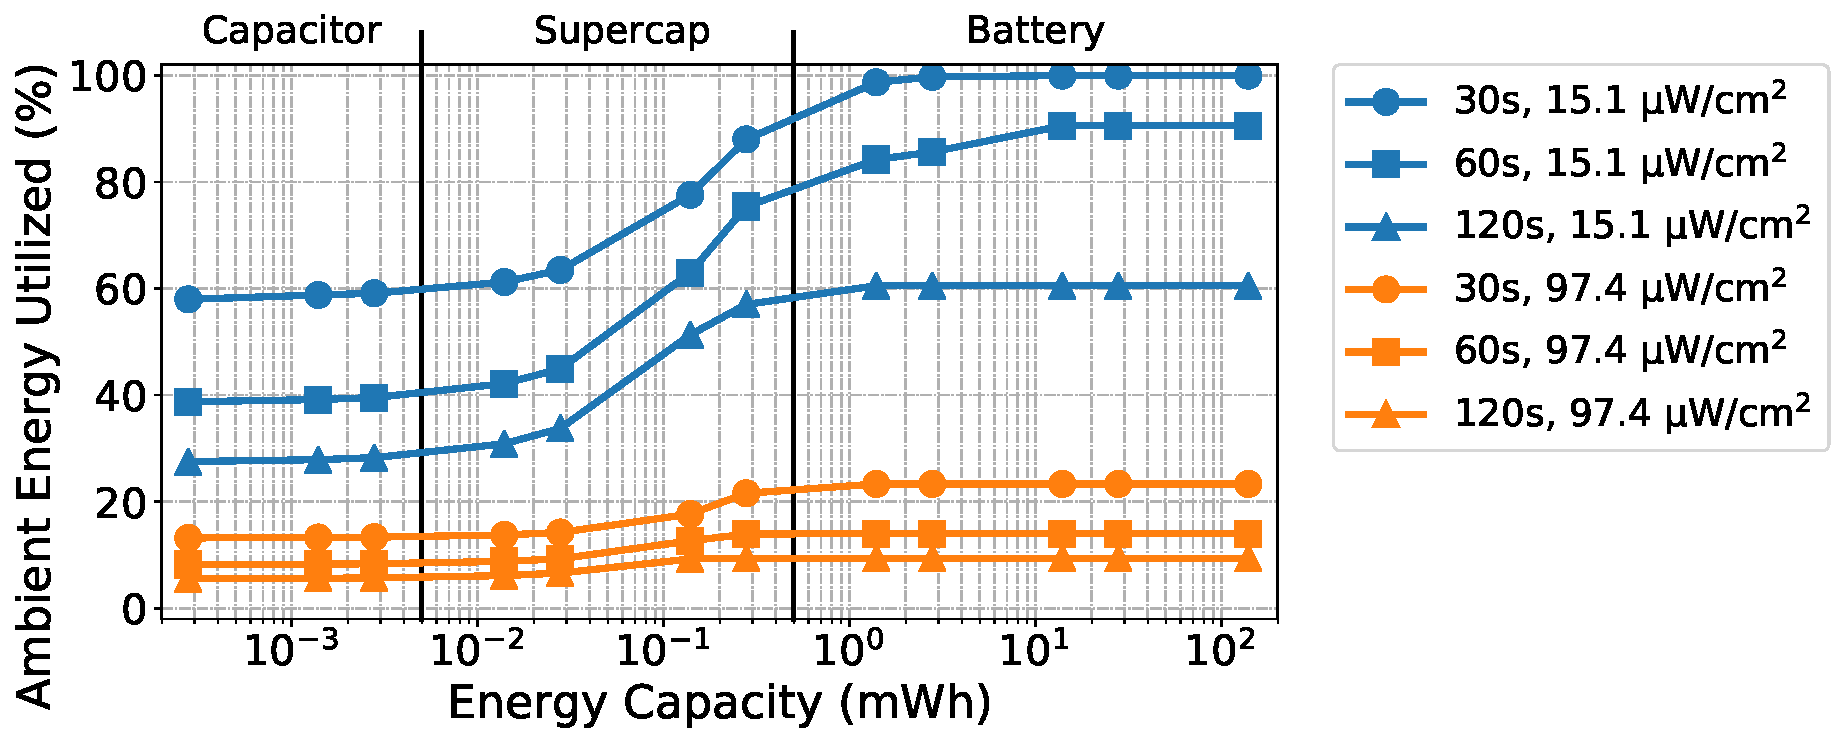
\includegraphics[width=0.9\linewidth]{figs/capacity/sense_and_send/usage_vs_secondary_size}
    \caption{Periodic application}
    \label{fig:usage:sensesec}
  \end{subfigure}
  \begin{subfigure}{0.49\textwidth}
    \centering
    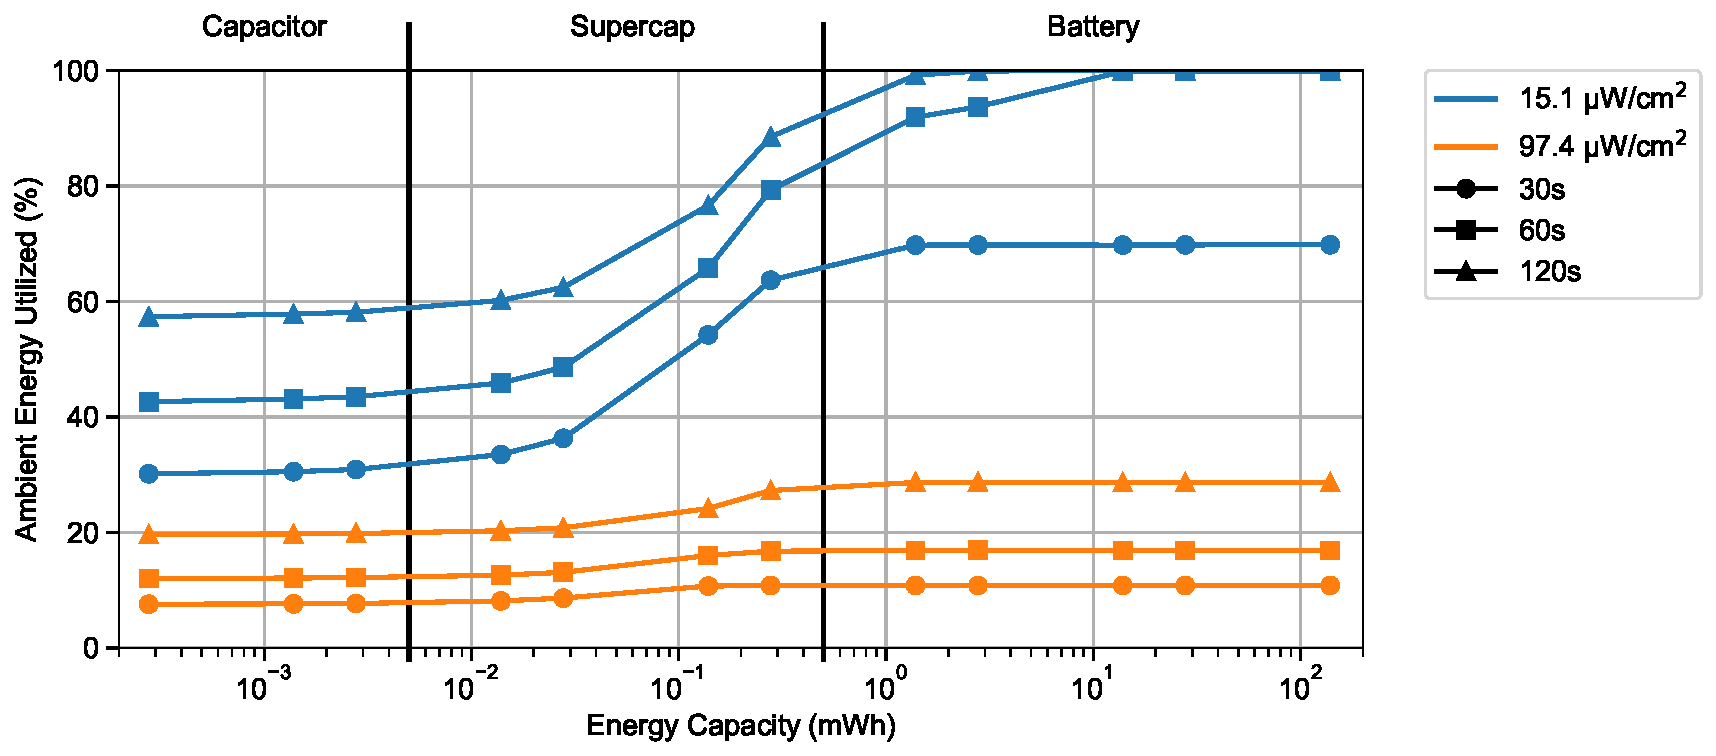
\includegraphics[width=0.9\linewidth]{figs/capacity/door_occupancy/usage_vs_secondary_size}
    \caption{Reactive application}
    \label{fig:usage:eventsec}
  \end{subfigure}
  \caption{\normalfont Ambient energy utilization
    as a function of idealized secondary storage capacity for different
    harvesting scenarios and workloads. The harvesting scenarios and workloads
    are described in \cref{sec:overview} and \cref{tab:rep}.  The x-axis is
    split by energy capacities possible with capacitors, supercapacitors, and
    batteries. The upper extents of capacity for (super)capacitors represent
    ten 100\,\si{\micro\farad} tantalum capacitors~\cite{tantalumDatasheet}, and one
    large 220\,mF supercapacitor~\cite{murataCap}. Larger capacitors exist, but
    are not appropriate for use on a small sensor node.  As energy storage increases, the harvestable energy used in
    the application also increases,
    %Increased energy utilization
    implying
    increased application performance.  Some scenarios, such as the periodic
    30\,s, 15.1\,\uW/cm\textsuperscript{2} case, reach 100\% utilization at
    high secondary capacities indicating that available energy is not
    sufficient to meet the application's requirements.
    %Most scenarios reach a
    %max utilization percentage that represents the amount of energy required by
    %each application.
    Generally, for both workloads and irradiance traces, from
    the smallest to largest capacity simulated, we see a 1.4-2.3x increase in
    utilized energy.
    %Even though the utilization percentage is not very high for
    %scenarios with high energy harvesting potential, even small increases in utilization
    %represent large increases in usable energy relative to the application's energy
    %requirements.
    }
\end{definefigure*}

\begin{definefigure*}{fig:reliability}
  \centering
  \begin{subfigure}{\textwidth}
    \begin{subfigure}{0.5\textwidth}
      \centering
      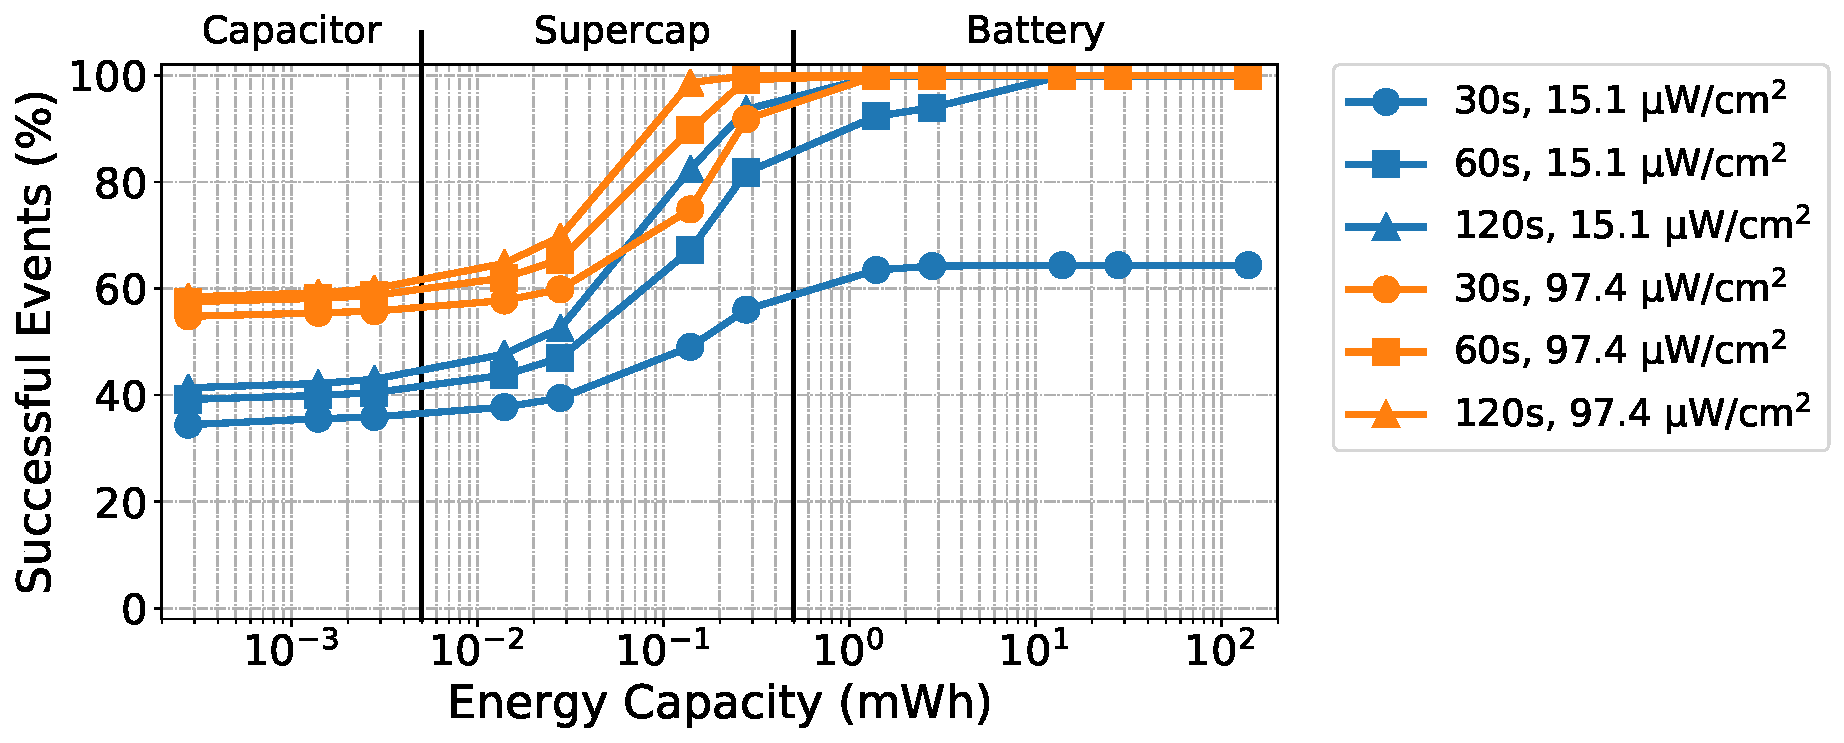
\includegraphics[width=0.9\linewidth]{figs/capacity/sense_and_send/events_vs_secondary_size}
        \caption{Periodic application}
      \label{fig:reliability:sensesec}
    \end{subfigure}
    \begin{subfigure}{0.5\textwidth}
      \centering
      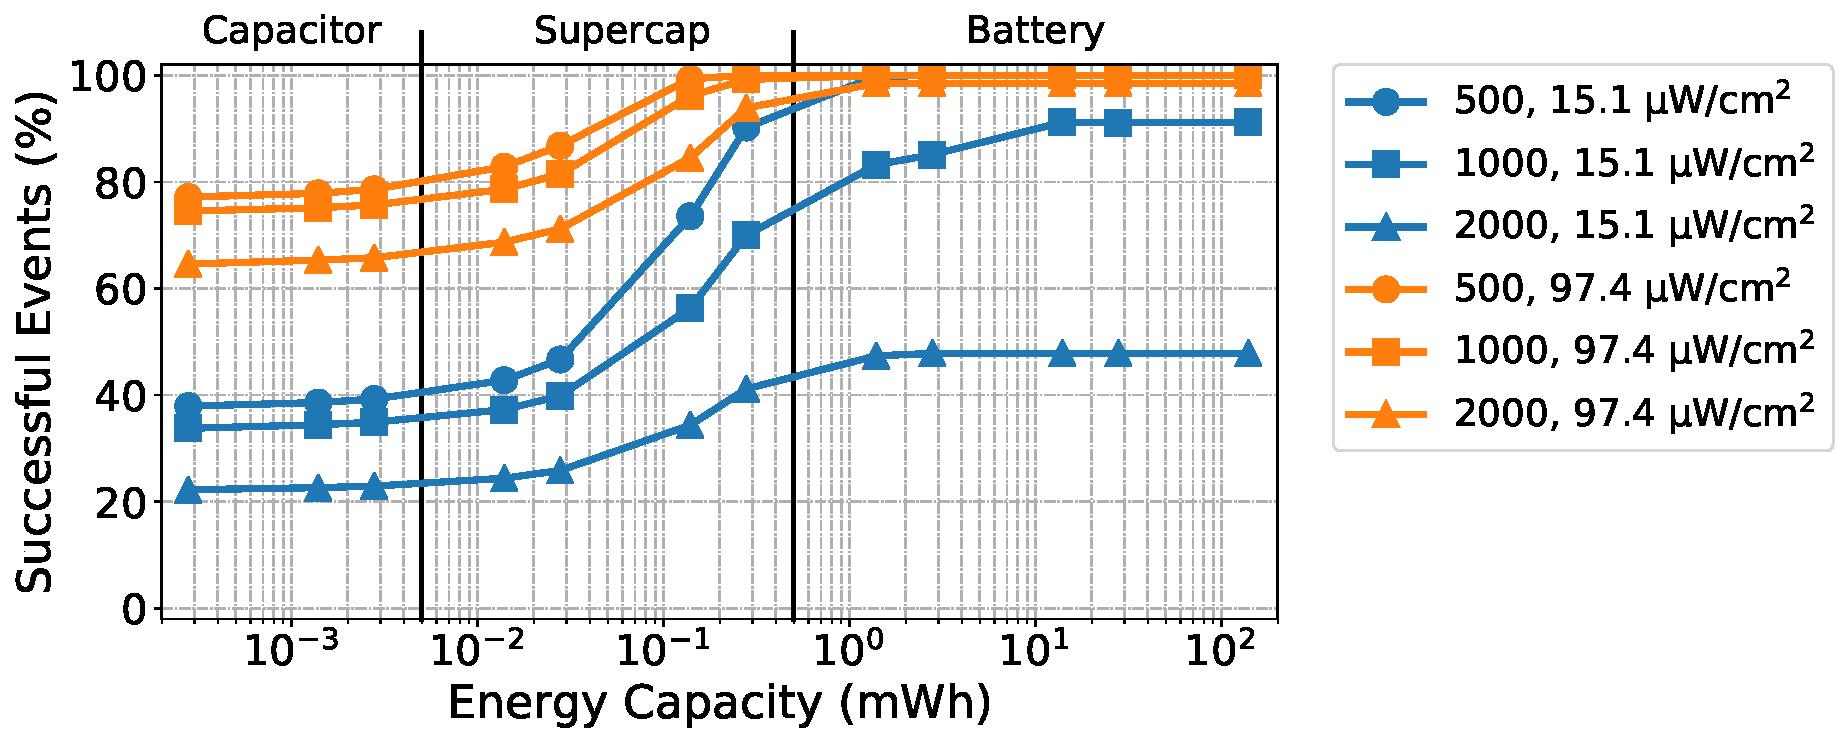
\includegraphics[width=0.9\linewidth]{figs/capacity/door_occupancy/events_vs_secondary_size}
      \caption{Reactive application}
      \label{fig:reliability:eventsec}
    \end{subfigure}
  \end{subfigure}
  \begin{subfigure}{\textwidth}
    \begin{subfigure}{0.5\textwidth}
      \centering
      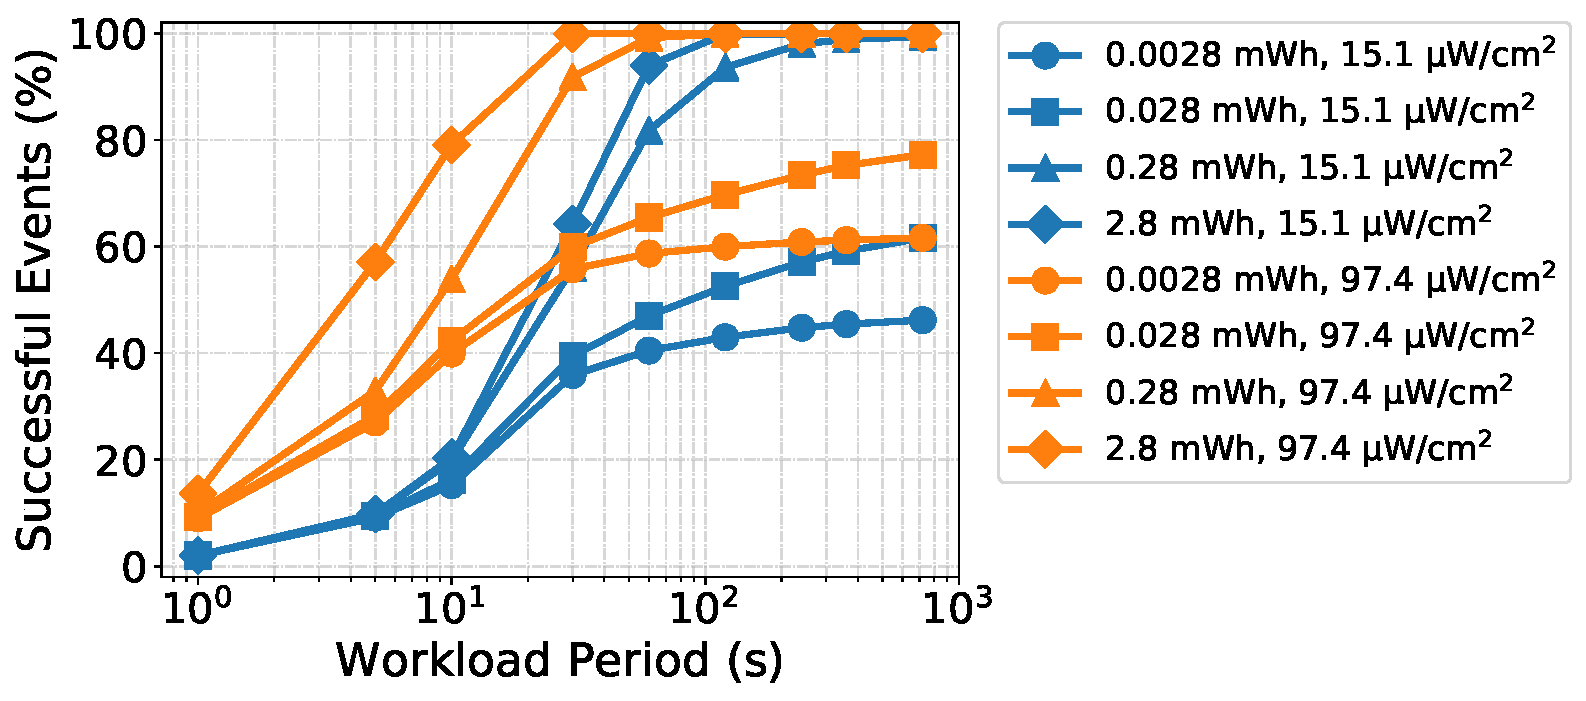
\includegraphics[width=0.9\linewidth]{figs/capacity/sense_and_send/events_vs_period}
      \caption{Periodic\textemdash varying period}
      \label{fig:reliability:senseper}
    \end{subfigure}
    \begin{subfigure}{0.5\textwidth}
      \centering
      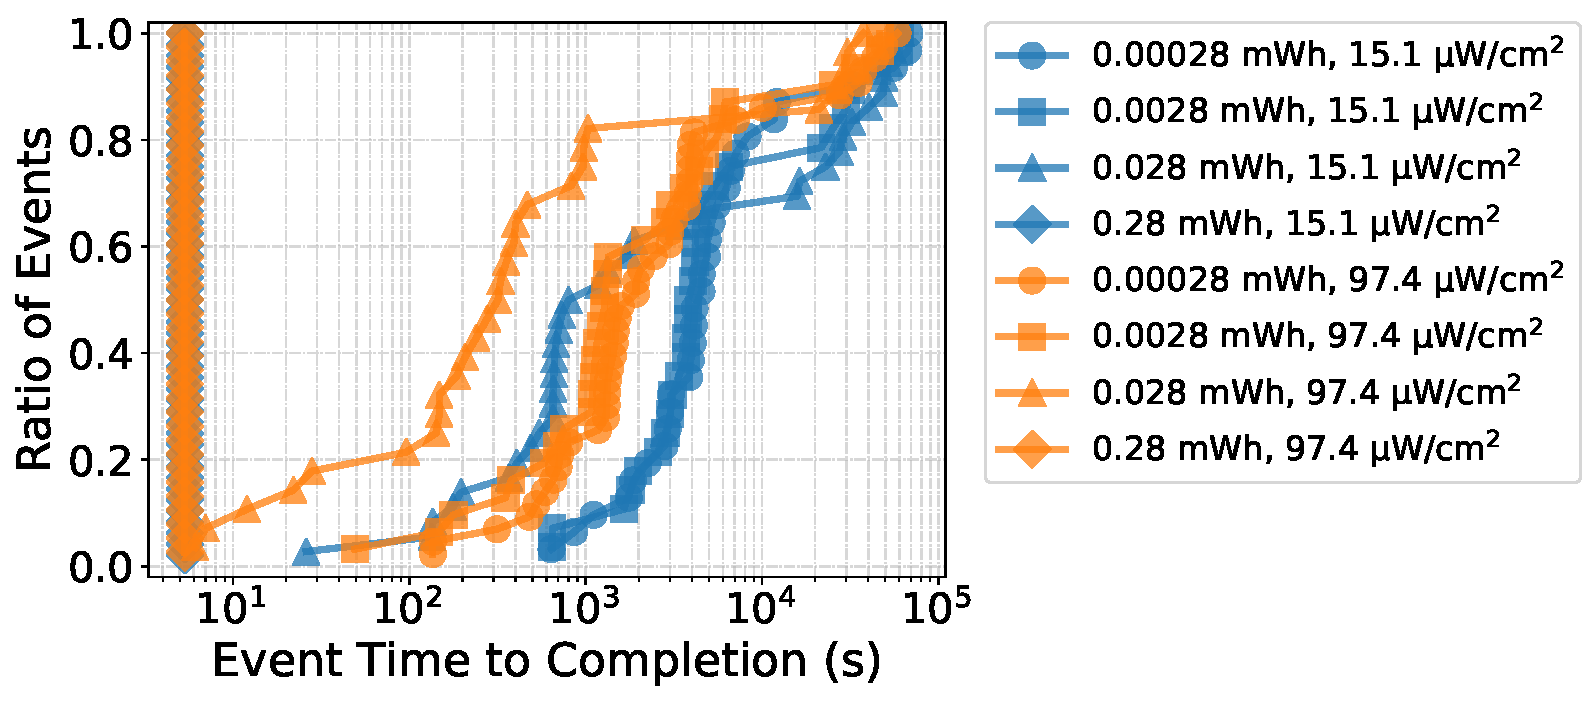
\includegraphics[width=0.9\linewidth]{figs/capacity/ota_update/ttc_ota}
      \caption{Long-running, high energy event}
      \label{fig:reliability:otattc}
    \end{subfigure}
  \end{subfigure}
  \caption{
    \normalfont
    Workload reliability
    for different harvesting scenarios, workloads, and idealized secondary storage sizes.
    We define reliability as the percentage of successfully completed events.
    %Systems are configured to
    %maximize this reliability, and must send a packet
    %within a specified period to be considered successful.
    As expected,
    workload reliability follows the same
    trend as energy utilization, improving with increased secondary energy
    storage. For both periodic and reactive workloads, from the smallest to
    largest capacity simulated, we see a 1.4-2.7x improvement in availability.
    In (c) we investigate the period at which different secondary storage sizes
    meet a specific reliability, showing that even with infrequent periodic
    workloads, small amounts of secondary storage have low reliability while
    larger secondary stores reach near 100\% reliability. (d) shows a CDF of
    time to completion for events in the long-running workload. In this
    workload, events are not atomic, and can be paused and resumed based on
    available energy. With secondary capacities that are large relative to the
    workload (which takes 93\,mJ) we see immediate completion.
    However, performing the event on smaller secondary capacities can take
    between three hours and a day to complete even for scenarios with large
    amounts of harvestable ambient energy.
    }
\end{definefigure*}